\documentclass[11pt,a4paper]{report}

\usepackage{microtype}
\usepackage[utf8]{inputenc}
%\usepackage{amsmath}
%\usepackage{amsfonts}
%\usepackage{amssymb}
\usepackage{float}
\usepackage{graphicx}
\graphicspath{{./images/}}
\usepackage[left=1.00cm, right=1.00cm, top=1.00cm, bottom=2.00cm]{geometry}
\author{Stéphane FEUGA\\{\small sfeuga@member.fsf.org}}
\title{{\Huge Rapport de Stage - Développeur Logiciel}\\
{\normalsize Stage du 02/04/2014 au 31/05/2014 pour l'association Uncanny}}
\date {En date du 29/04/2014}
\begin{document}

\maketitle

\vspace*{\stretch{1}}
\begin{center}
This page intentionally left blank
\footnotetext{Ce document est rédigé avec \LaTeX}
\thispagestyle{empty}
\end{center}
\vspace*{\stretch{1}}

\tableofcontents

\chapter{Présentation}
	\section{Introduction}
		\paragraph*{}
	\section{Historique}
		\paragraph*{}
	\section{L'Association Uncanny}
		\paragraph*{}
	\section{Compétences à mettre en œuvre}
		\paragraph*{\indent Compétence Obligatoire :} Développer une interface utilisateur.
		\paragraph*{\indent Compétence Choisie :} Mettre en œuvre une solution de gestion de contenu ou d’e-commerce.
	\section{Remerciements}
		\paragraph*{}Tout d'abord, je souhaite  remercier Mr Cédric CHERDEL et Mr Laurent CEBE de l'association Uncanny qui m'ont offert la possibilité d'avoir un sujet de stage en adéquation avec mes capacités et les compétences à mettre en œuvre pour la validation de ce stage.
		\paragraph*{}Je souhaite aussi remercier Gabriel BLOCK, Emanuelle FERRAND, Erwan FOURNEL et Florence \linebreak NATIVELLE (tous de l'I.M.I.E.) pour leurs implications dans cette formation.
		\paragraph*{}Je souhaite enfin remercier ma femme Akané et Ada Lovelace\footnote{https://fr.wikipedia.org/wiki/Ada\_Lovelace} sans qui nous ne serions pas là.

\chapter{Mission}
	\section{Présentation du projet}
		Le projet est la mise en place de deux sites internet pour promouvoir les projets et activités de l'association Uncanny. 
		\subsection{Objectifs}
			\begin{enumerate}
				\item Une page d'accueil animé donnant accès aux contenues.\\
				Cette page sera en HTML5 et responsive.
				\item Création d'un thème responsive en HTML5 pour Wordpress.
				\item Un site internet sur la production de danse contemporaine.\\
				Mise en place d'un Wordpress.
				\item Un site lié à l'activité de massage THAÏ.\\
				Mise en place d'un Wordpress.
			\end{enumerate}
		\subsection{Cible}
			\begin{itemize}
				\item Les professionnels de la Danse
				\item Les particuliers
				\item Les compagnies de Danse
				\item Les Mairies
				\item Les Départements et Régions
			\end{itemize}
		\subsection{Les acteurs}
			\begin{itemize}
				\item Cédric CHERDEL
				\item Laurent CEBE
			\end{itemize}
		\subsection{L'existant}
			\begin{enumerate}
				\item Une charte Graphique
				\item Une liste de contact
				\item Des documentations sur les projets de danse
			\end{enumerate}
	\section{Fonctionnalités \& Contraintes}
		\paragraph*{}
	\section{L'Expérience Utilisateur et l'Accessibilité}
		\subsection{Le Maquettage}
			\paragraph*{Zoning}\subparagraph*{}
				\begin{figure}[H]
					\centering
					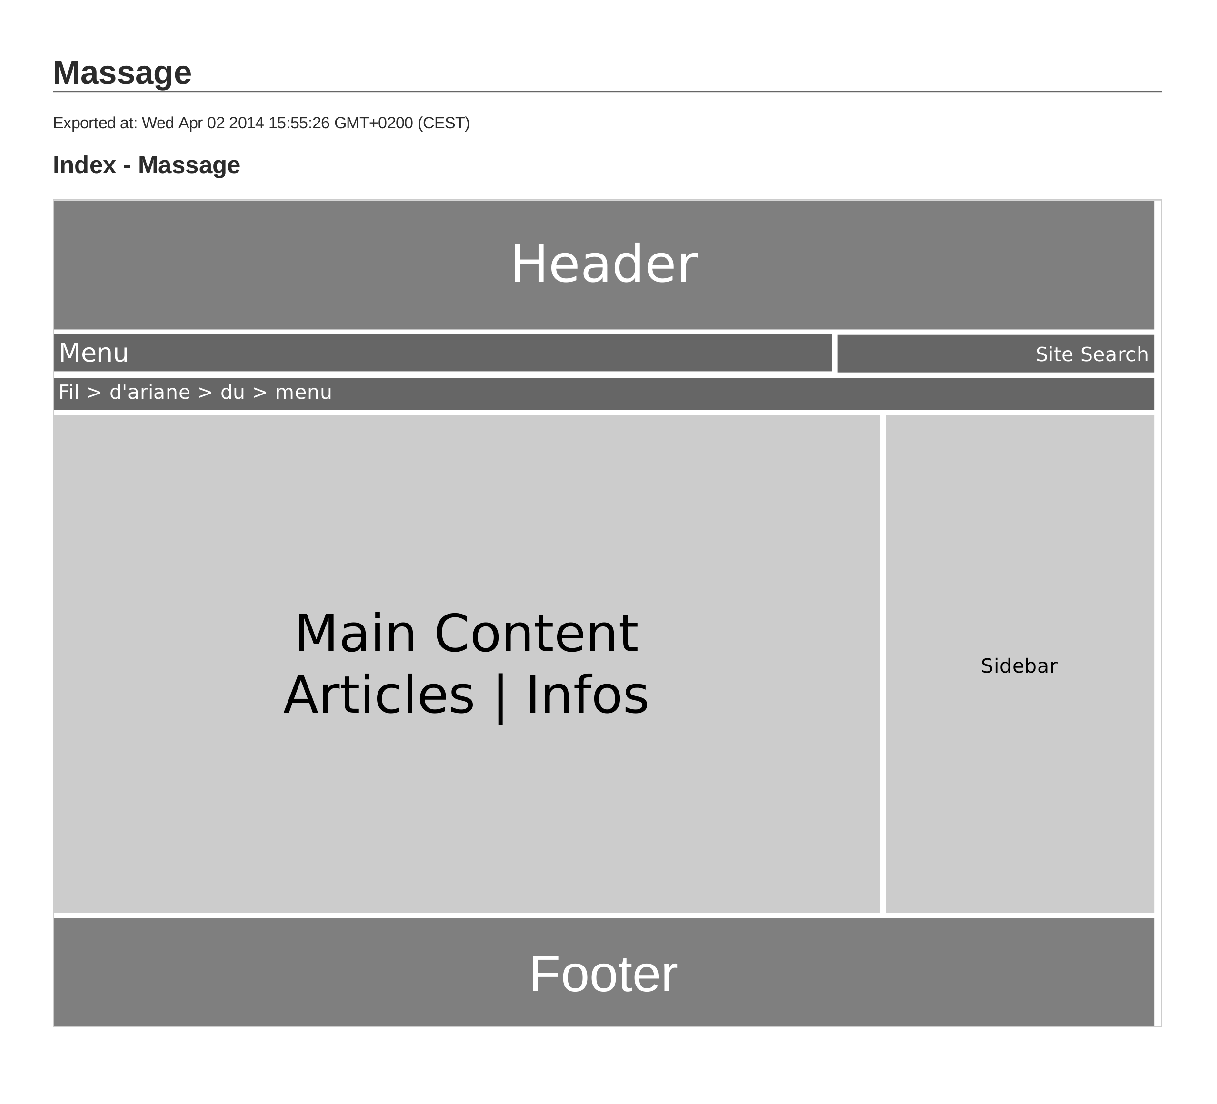
\includegraphics[height=10cm]{Zone-Massage.eps}
					\caption{Zoning du site "Massage"}
					\label{fig:Zoning-Massage}
				\end{figure}
				\begin{figure}[H]
					\centering
					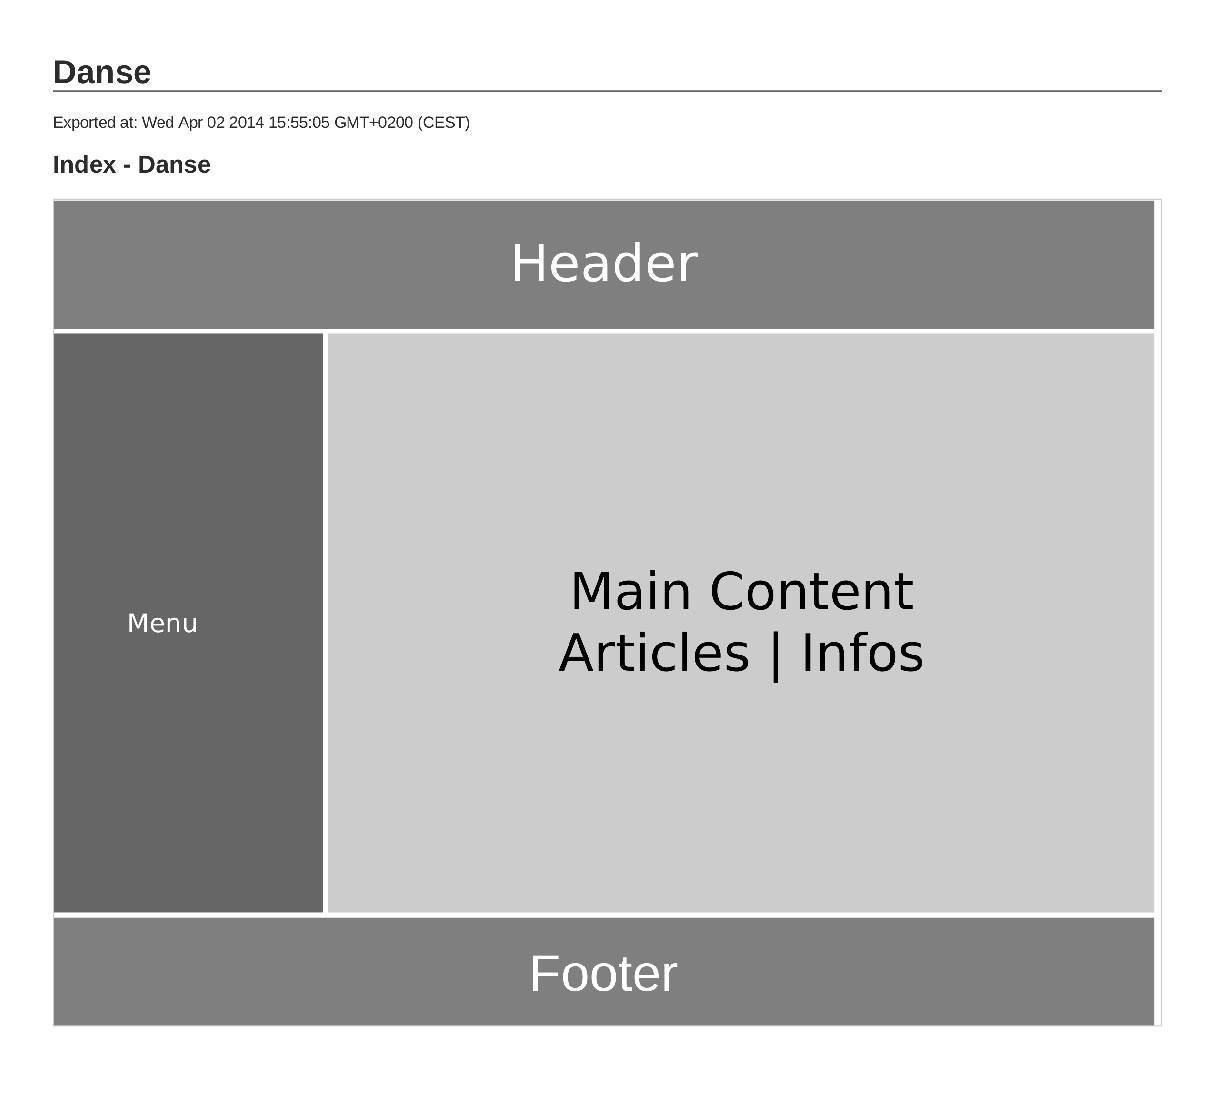
\includegraphics[height=10cm]{Zone-Danse.eps}
					\caption{Zoning du site "Danse"}
					\label{fig:Zoning-Danse}
				\end{figure}

			\paragraph*{Wireframe}\subparagraph*{}
				\begin{figure}[H]
					\centering
					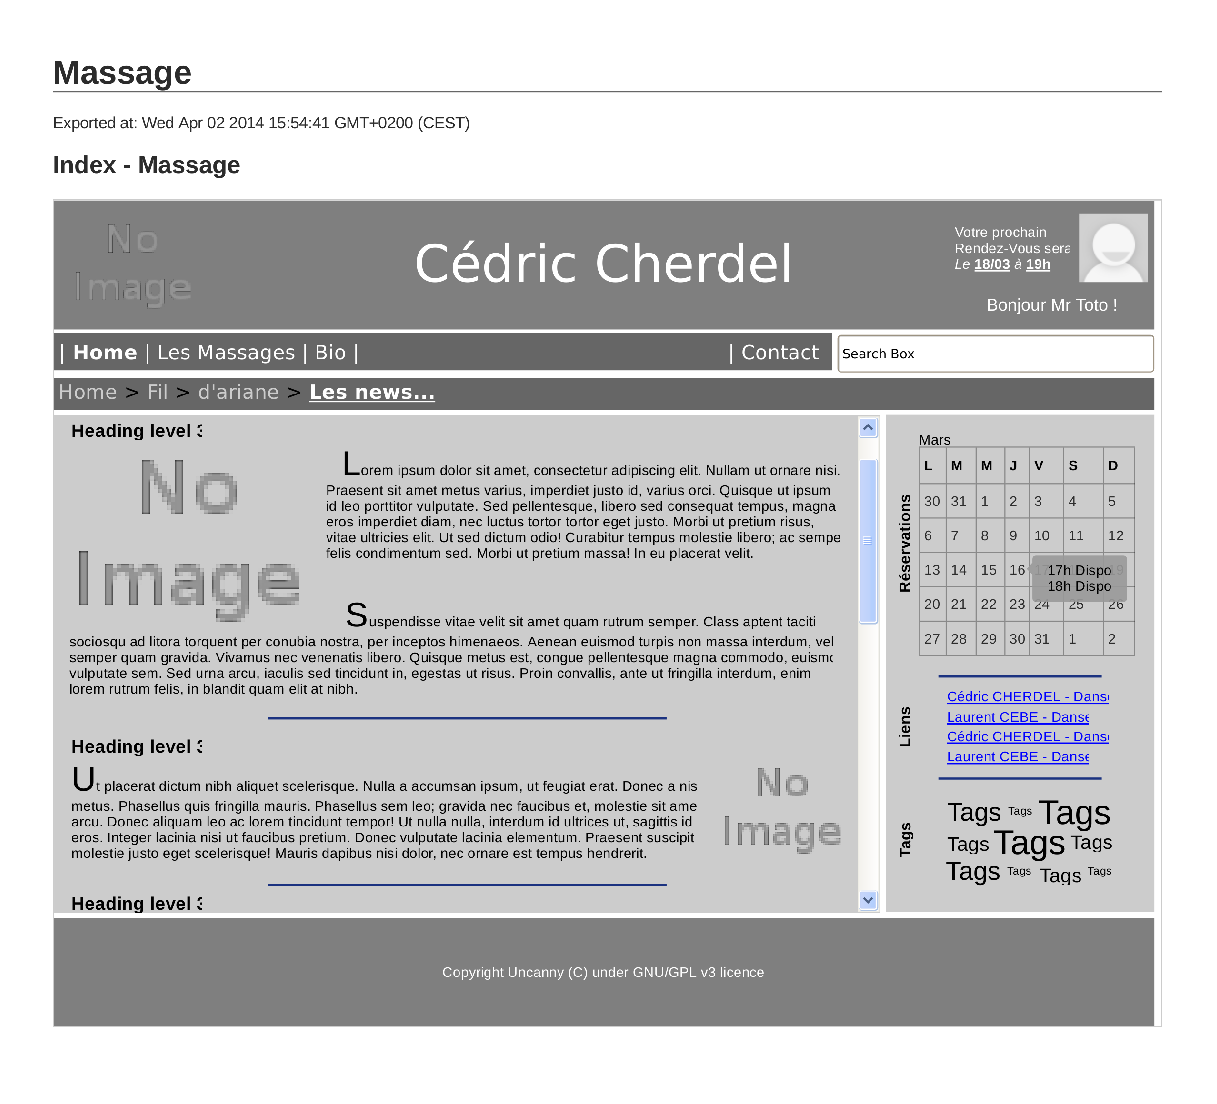
\includegraphics[height=10cm]{Wireframe-Massage_1.eps}
					\caption{Wireframe du site "Massage"}
					\label{fig:Wireframe-Massage_1}
				\end{figure}
				\begin{figure}[H]
					\centering
					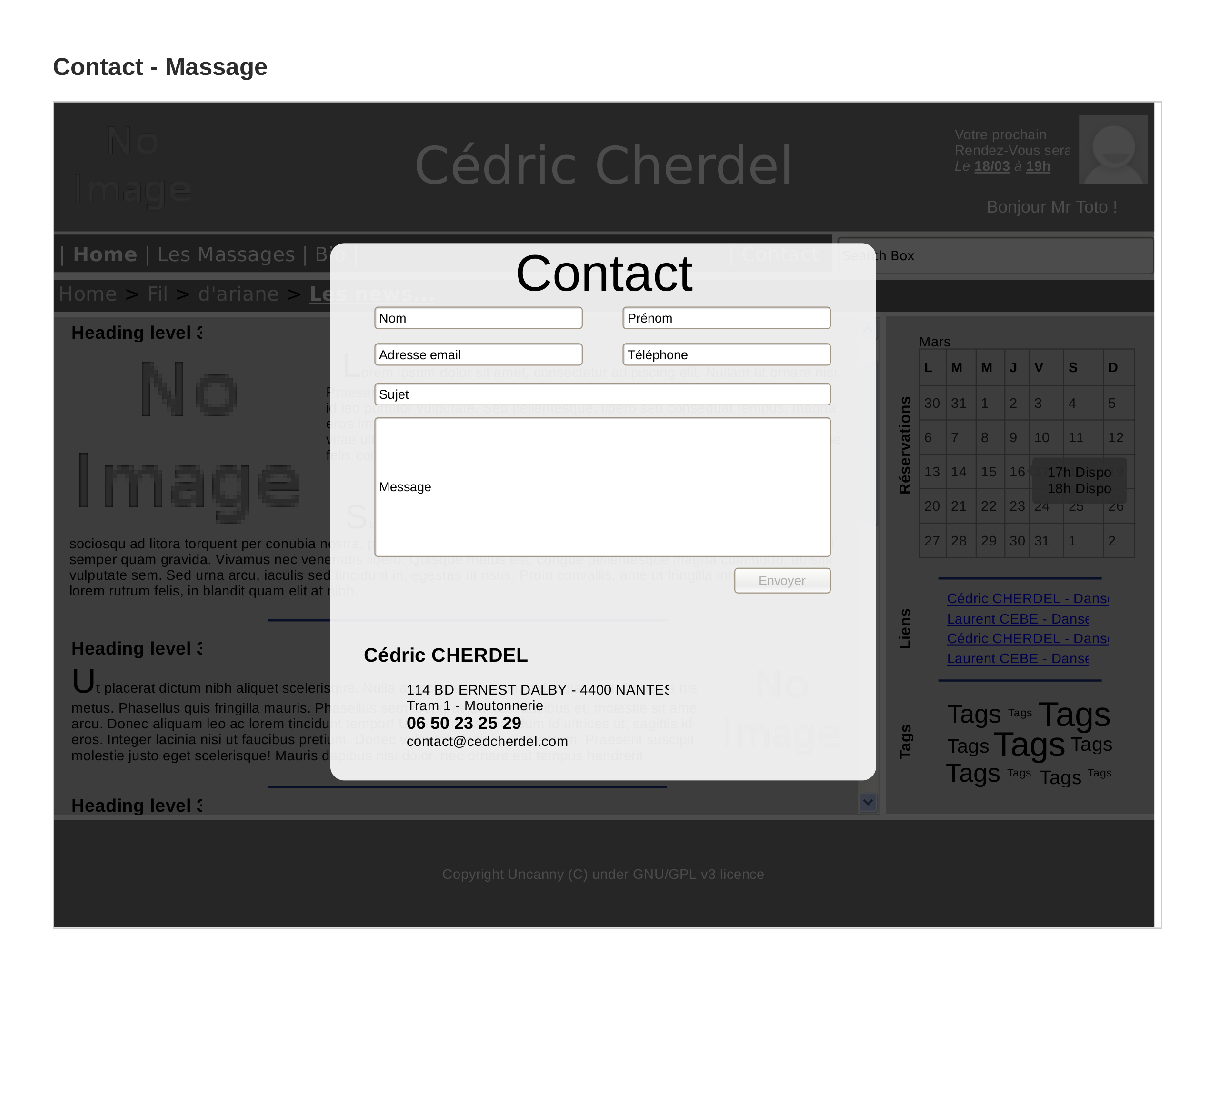
\includegraphics[height=10cm]{Wireframe-Massage_2.eps}
					\caption{Site "Massage": Exemple de Pop-In}
					\label{fig:Wireframe-Massage_2}
				\end{figure}
				\begin{figure}[H]
					\centering
					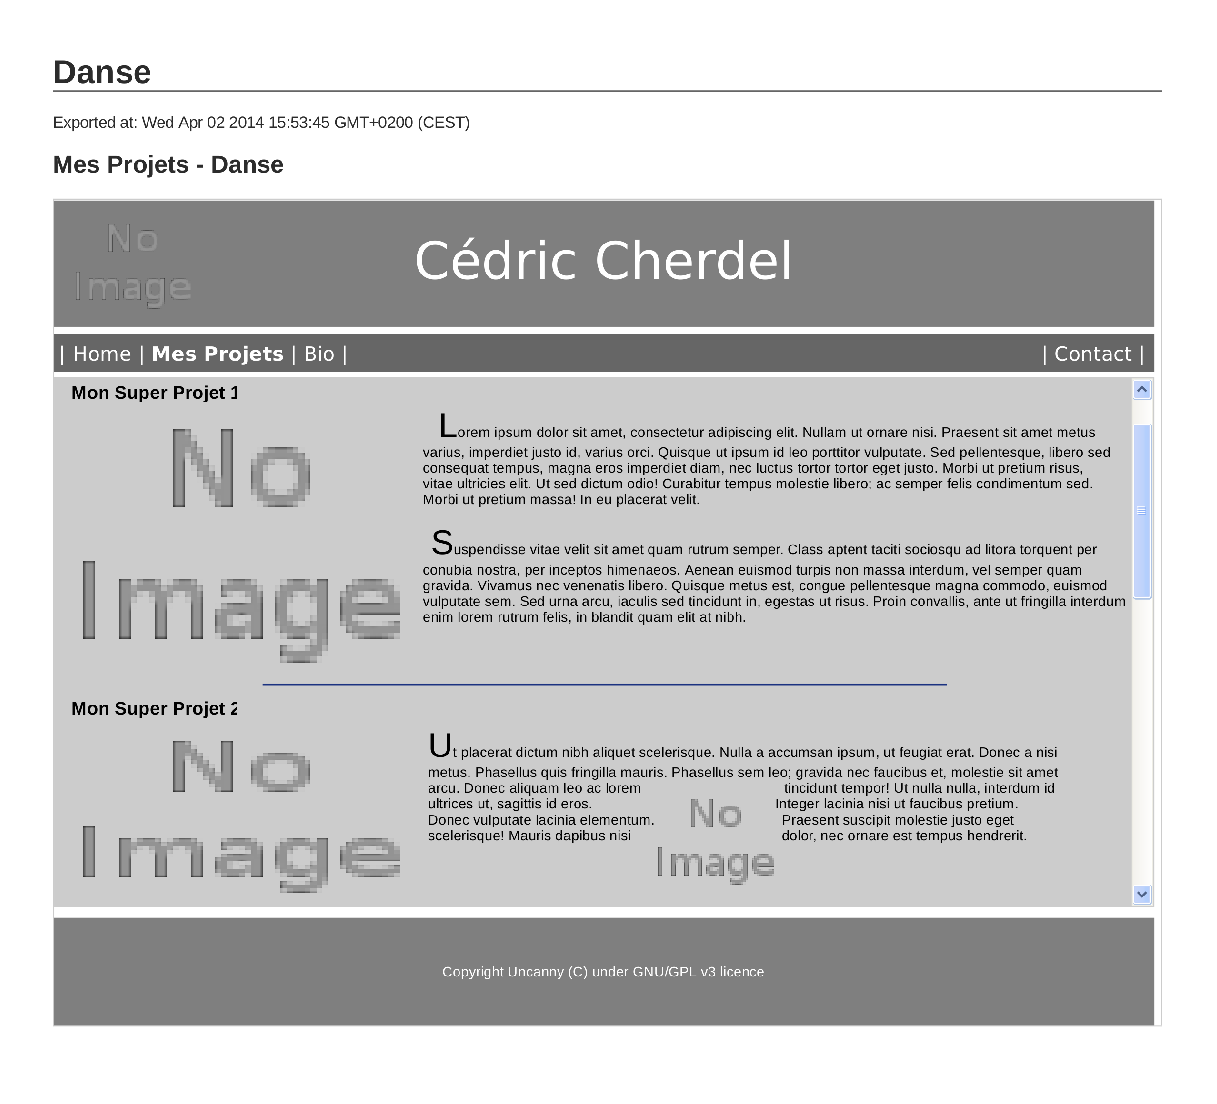
\includegraphics[height=10cm]{Wireframe-Danse_1.eps}
					\caption{Wireframe du site "Danse"}
					\label{fig:Wireframe-Danse_1}
				\end{figure}
				\begin{figure}[H]
					\centering
					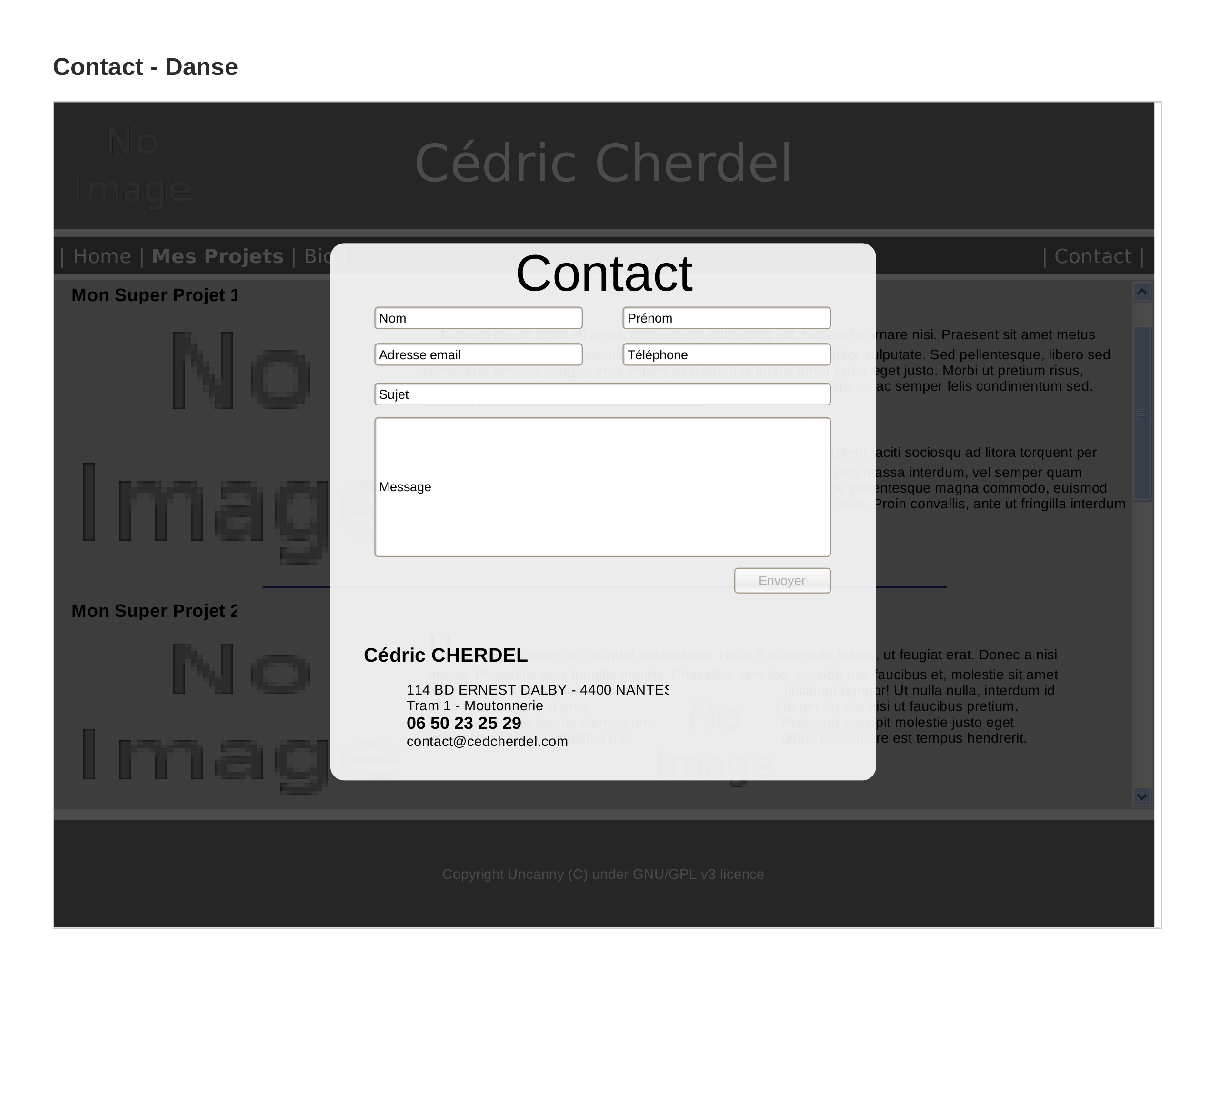
\includegraphics[height=10cm]{Wireframe-Danse_2.eps}
					\caption{Site "Danse": Exemple de Pop-In}
					\label{fig:Wireframe-Danse_2}
				\end{figure}

			\paragraph*{Prototype}\subparagraph*{}
				\begin{figure}[H]
					\centering
					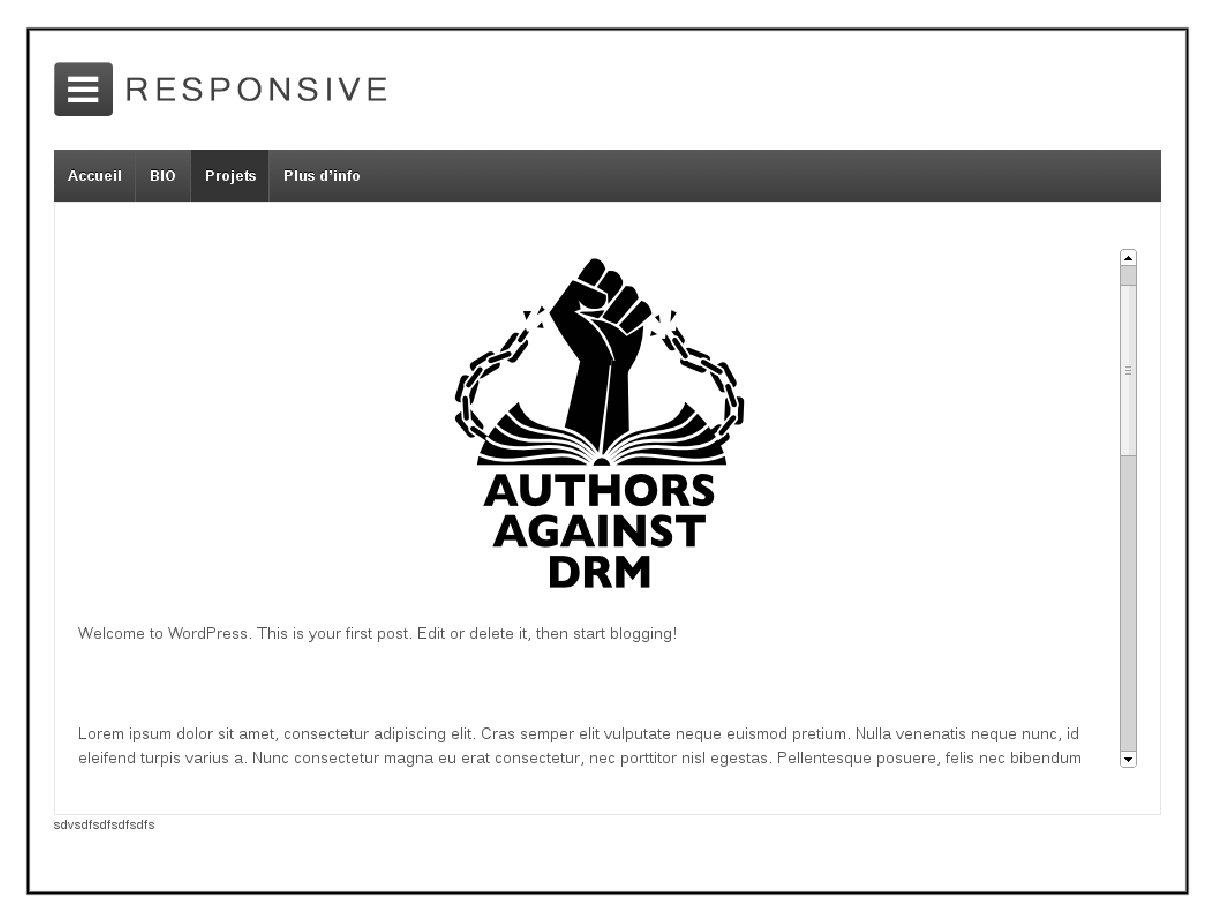
\includegraphics[height=10cm]{Prototype-Wordpress.eps}
					\caption{Prototype du site "Danse"}
					\label{fig:Prototype-Wordpress}
				\end{figure}

			\paragraph*{Mood Board, Styles Tiles \& Mockup}\subparagraph*{}
				\begin{figure}[H]
					\centering
					
\includegraphics[height=10cm]{Mockup-Danse_1.eps}
					\caption{Mockup page d'accueil du site "Danse"}
					\label{fig:Mockup-Danse_1}
				\end{figure}
				\begin{figure}[H]
					\centering
					
\includegraphics[height=10cm]{Mockup-Danse_2.eps}
					\caption{Mockup page projets du site "Danse"}
					\label{fig:Mockup-Danse_2}
				\end{figure}

	\section{Planning: méthodes et outils}
		\subsection{Cahier des charges}
			\paragraph*{}J'ai commencé par rédiger un premier cahier des charge vierge (basé sur un modèle fournie par l'I.M.I.E.). Lors du premier jours, j'ai expliqué rapidement l'utilité d'un cahier des charge, puis dans une deuxièmes réunion, nous avons échangés autour des questions destiné à remplir ce cahier des charge. Enfin, lors de la réunion de validation, nous avons repris tout les points afin de les valider. Vous le trouverez en annexe 6.
		\subsection{WBS, Pert \& Gantt}
			\paragraph*{}Les Pert et Gantt sont réalisé en ligne via Gantter\footnote{http://www.gantter.com} (application intégré dans Google Drive).
			\paragraph*{WBS}...-Manque le ScreenShot-...
			\paragraph*{Pert}...-Manque le ScreenShot-...
			\paragraph*{Gantt}...-Manque le ScreenShot-...
		\subsection{Agilité, Kanban Board \& Git}
			\paragraph*{}Nous avons choisi de travailler en Agilité. Les Sprints sont d'une semaine et ne se rapport qu'à une fonctionnalité. Nous utilisons intensivement un Kanban Board\footnote{http://tsu3d.hestia.feralhosting.com/kanban} ainsi que les outils Google Drive pour le partage et la présentation des fonctionnalités.
			\paragraph*{}Ce mode de fonctionnement m'as permis d'avoir un grande réactivité lors de changement important et l'utilisation du Kanban Board à permis à toutes les parties prenantes de suivre l'avancement du projet au jour le jour.
			\begin{figure}[H]
				\centering
				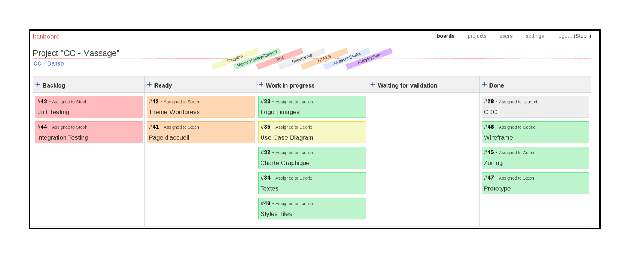
\includegraphics[width=\textwidth]{kanban.eps}
				\caption[Kanban Board]{Exemple d'utilisation du Kanban Board pour le site "Massage"}
				\label{fig:Kanban-Board}
			\end{figure}
			\paragraph*{}Enfin, l'utilisation de GIT (avec Gitorious\footnote{https://gitorious.org/uncanny}) fut aussi intensive. Plusieurs Repository ont été créé pour partager (et garder une trace des modifications) aussi bien les différents codes sources des sites, que les documentations, le cahier des charge (et ses annexes) ainsi que ce rapport. Ça a permis à tout le monde d'avoir accès à tout et de pouvoir suivre les modifications.
			

\chapter{Conception}
	\section{Modélisations UML}
			\subsection{Use Case}\paragraph*{}
			\begin{figure}[H]
				\centering
				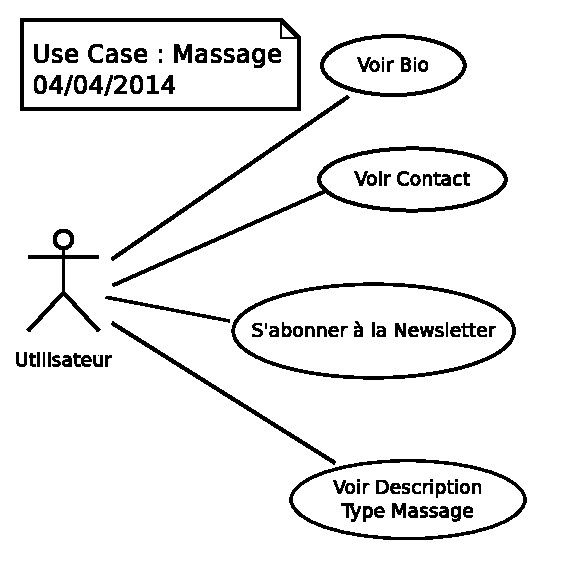
\includegraphics[height=10cm]{UseCase-Massage-User.eps}
				\caption[Use Case Utilisateur Massage]{Use Case d'un Utilisateur pour le site "Massage"}
				\label{fig:UseCase-Massage_User}
			\end{figure}
			\begin{figure}[H]
				\centering
				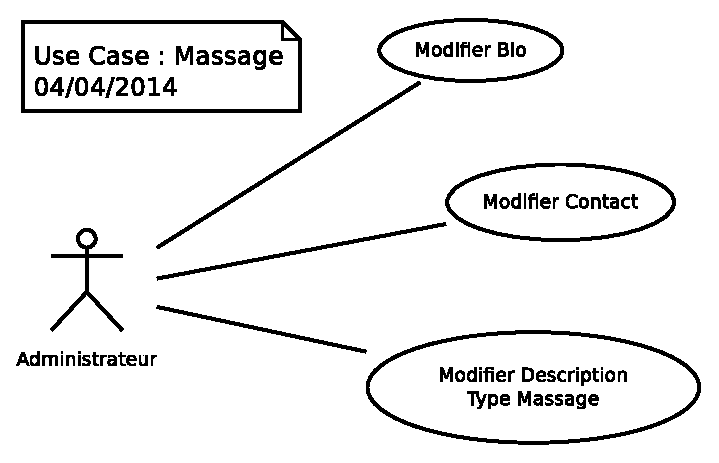
\includegraphics[height=10cm]{UseCase-Massage-Administrateur.eps}
				\caption[Use Case Administrateur Massage]{Use Case de l'administrateur pour le site "Massage"}
				\label{fig:UseCase-Massage_Admin}
			\end{figure}
			\begin{figure}[H]
				\centering
				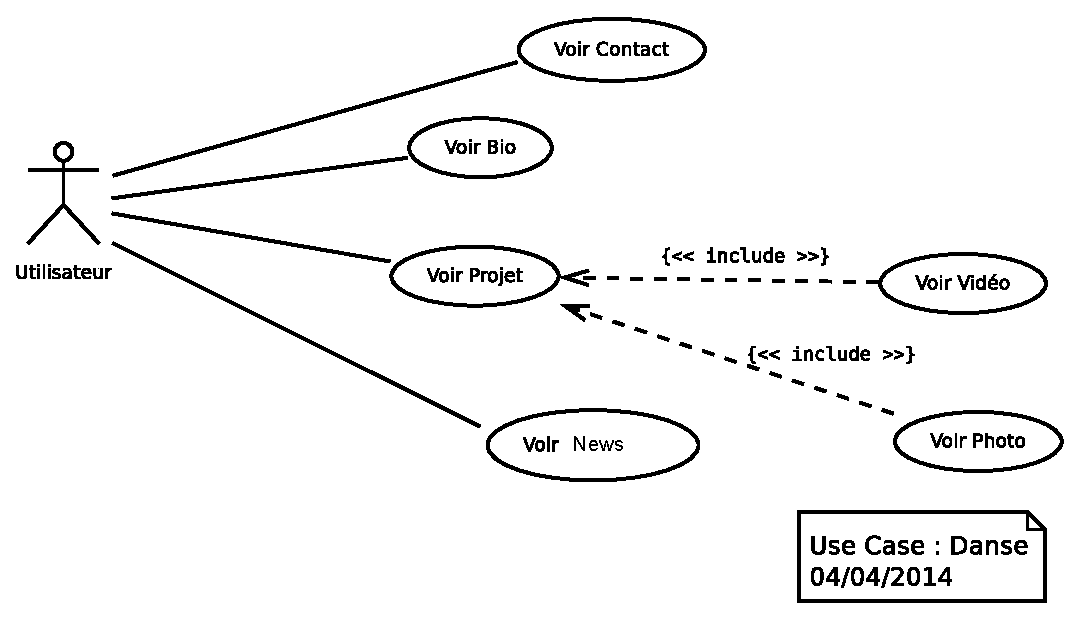
\includegraphics[height=10cm]{UseCase-Danse-User.eps}
				\caption[Use Case Utilisateur Danse]{Use Case d'un Utilisateur pour le site "Danse"}
				\label{fig:UseCase-Danse_User}
			\end{figure}
			\begin{figure}[H]
				\centering
				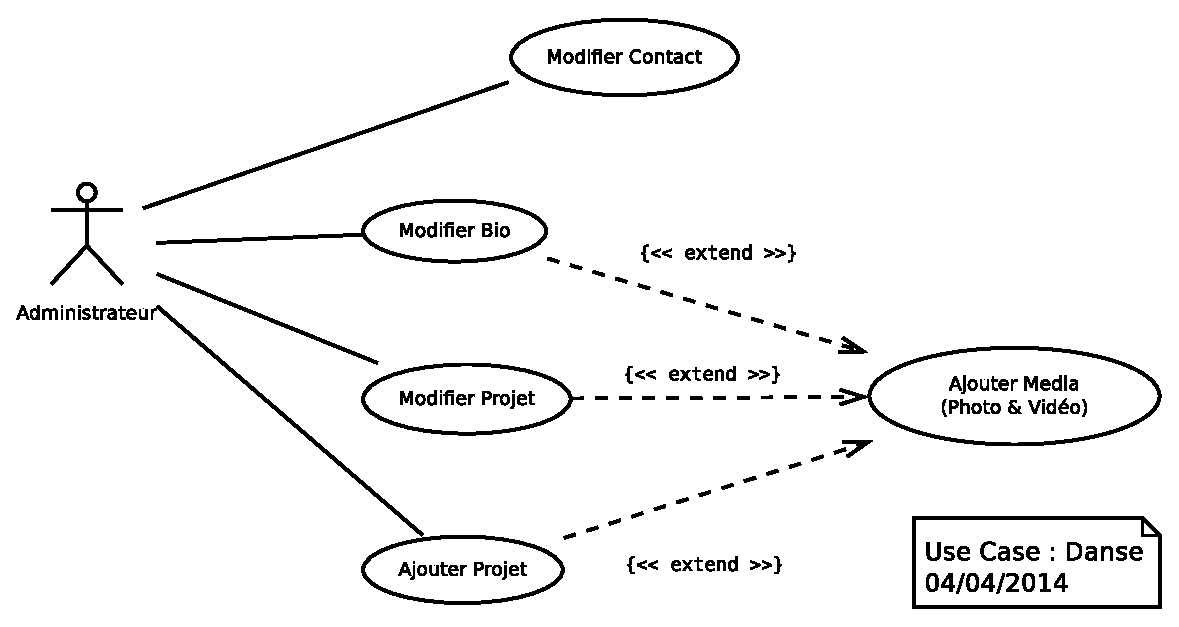
\includegraphics[height=10cm]{UseCase-Danse-Administrateur.eps}
				\caption[Use Case Administrateur Danse]{Use Case de l'administrateur pour le site "Danse"}
				\label{fig:UseCase-Danse_Admin}
			\end{figure}
				
	\section{Test \& Qualité}
		\subsection{Fonctionnel}
		\subsection{Intégration}

\chapter{Développement}
	\section{Technologies}
		\subsection{Page d'accueil}
			\paragraph{Pages HTML}
			\paragraph{CSS \& Responsive Design}
		\subsection{Thème}
			\paragraph{php}
			\paragraph{CSS \& Responsive Design}

\chapter{Déploiement \& Recette}
	\section{Prérequis techniques}
		\paragraph{}Un serveur web avec PHP 5.2.4 ou plus, MySQL 5.0 ou plus, le module Apache mod\_rewrite et un accès FTP.
	%\section{Scripts de mise en place de l'architecture logiciels}
	%\section{Scripts de déploiement de l'application}
	\section{Documentation:}
		\subsection{Développeur}Tout le code spécifique à été commenté. L'utilisation des documentations officiels de Wordpress\footnote{https://codex.wordpress.org}, de Less\footnote{http://lesscss.org}, de jQuery\footnote{http://api.jquery.com}, jQuery UI\footnote{http://api.jqueryui.com} ainsi que de php\footnote{http://www.php.net/manual/en/index.php} sont aussi vivement recommandé.
		\subsection{Administrateur}Une documentation sur l'administration générale et l'ajout de projet est disponible en annexe 7.
	\section{Recette}

\chapter{Bilan \& Conclusion}
	\paragraph*{}Ce stage m'as permis d'acquérir de nouvelles compétences aussi bien au niveau théorique que pratique. J'ai pu améliorer mes connaissances sur Wordpress et sur HTML5. Enfin, j'ai découvert le monde de la Danse contemporaine ainsi que les éléments nécessaires à la mise en place d'un spectacle.
	\paragraph*{}En effet, cette période de deux mois au sein de cette association m'a permis:
	\begin{itemize}
		\item De mieux connaitre le milieu associatif
		\item D'étendre mes connaissances acquises lors de la formation en réalisant un thème Wordpress en tenant compte des contraintes de mis en pages sur différentes plateformes
		\item D'utiliser les nouveautés d'animation en HTML5 pour la pages d'accueil
		\item De me familiariser avec les canvas HTML5 et plus généralement le SVG
		\item D'utiliser les librairies jQuery et jQuery UI
		\item D'avoir une meilleur vision des contraintes lié à un développement spécifique
	\end{itemize}
	\paragraph*{}La réalisation de ces tâches, l'aide de la communauté Wordpress France et l'implication des différents acteurs de ce stage, m'a permis d'atteindre les objectifs demandés, de devenir plus autonome et opérationnel dans le développement web, d'exploiter mes connaissances et dans acquérir de nouvelles.
	\paragraph*{}Pour finir, je suis convaincu que cette expérience me permettra d'être en adéquation avec le marché de l'emploi dans la région.
	

%\chapter*{Lexique}

\chapter{Liste des Annexes}
	\begin{enumerate}
		\item CV
		\item Contenu pédagogique
		\item Présentation du titre
		\item RC
		\item REAC
		\item Cahier des Charges
		\item Documentation Administrateur
	\end{enumerate}


\listoffigures \pagenumbering{Roman}
\listoftables

\end{document}
